% --------------------------- INTRODUCTION ----------------------------
\section{Introduction}
\label{sec:intro}

The shift from active to passive equity management is structural \parencite{financialtimes-active-to-passive,jpmorgan-exchange-traded-funds-etfs}: passive assets under management have surpassed active in the United States, and DNB Asset Management launched Norway's first dedicated enhanced-index equity fund in 2023 \parencite{dnb-global-enhanced-index}. Enhanced-index investors live in a narrow tracking-error band around a benchmark and search for small, repeatable sources of alpha \parencite{riepe-werner-are-enhanced-index-mutual-funds-worthy-of-their-name,jorion-enhanced-index-funds-and-tracking-error-optimization}. One of the oldest such sources is the \emph{index effect} of \textcite{shleifer-do-demand-curves-for-stocks-slope-down}: stocks added to a benchmark earn abnormal returns in the days surrounding their effective inclusion, while deletions earn the symmetric loss. \textcite{lynch-new-evidence-s&p-500} document the effect on the S\&P~500, \textcite{afego-effects-of-changes-in-stock-index-composition} on a wide cross-section of indices, and \textcite{nbim-investing-in-equities} describe Norges Bank Investment Management's well-known internal index-event programme on global benchmarks.

For OSEBX --- the 50--80 stock benchmark of the Oslo Stock Exchange, rebalanced semi-annually from a publicly-disclosed selection rule \parencite{OSEBX-rule-book} applied to the $\sim$200-stock OSEAX universe --- the index effect has been documented \parencite{cbs-thesis-price-and-volume-effects-osebx,nhh-thesis-exploiting-the-index-effect-to-extract-alpha} but, to our knowledge, never \emph{traded} in an out-of-sample, simulation-based study that anticipates the announcement date. Figure~\ref{fig:idxeff} illustrates the effect on aggregate: from 2002 to 2023, future additions trend up and future deletions trend down in the weeks before the effective date (day 0), with a partial mean reversion afterwards. The rebalancing timeline has three dates --- cut-off date (CD), announcement date (AD), and effective date (ED) --- and the trading window of interest sits between the cut-off and the announcement, when constituent data is fixed but not yet public.

\begin{figure}[H]
\centering
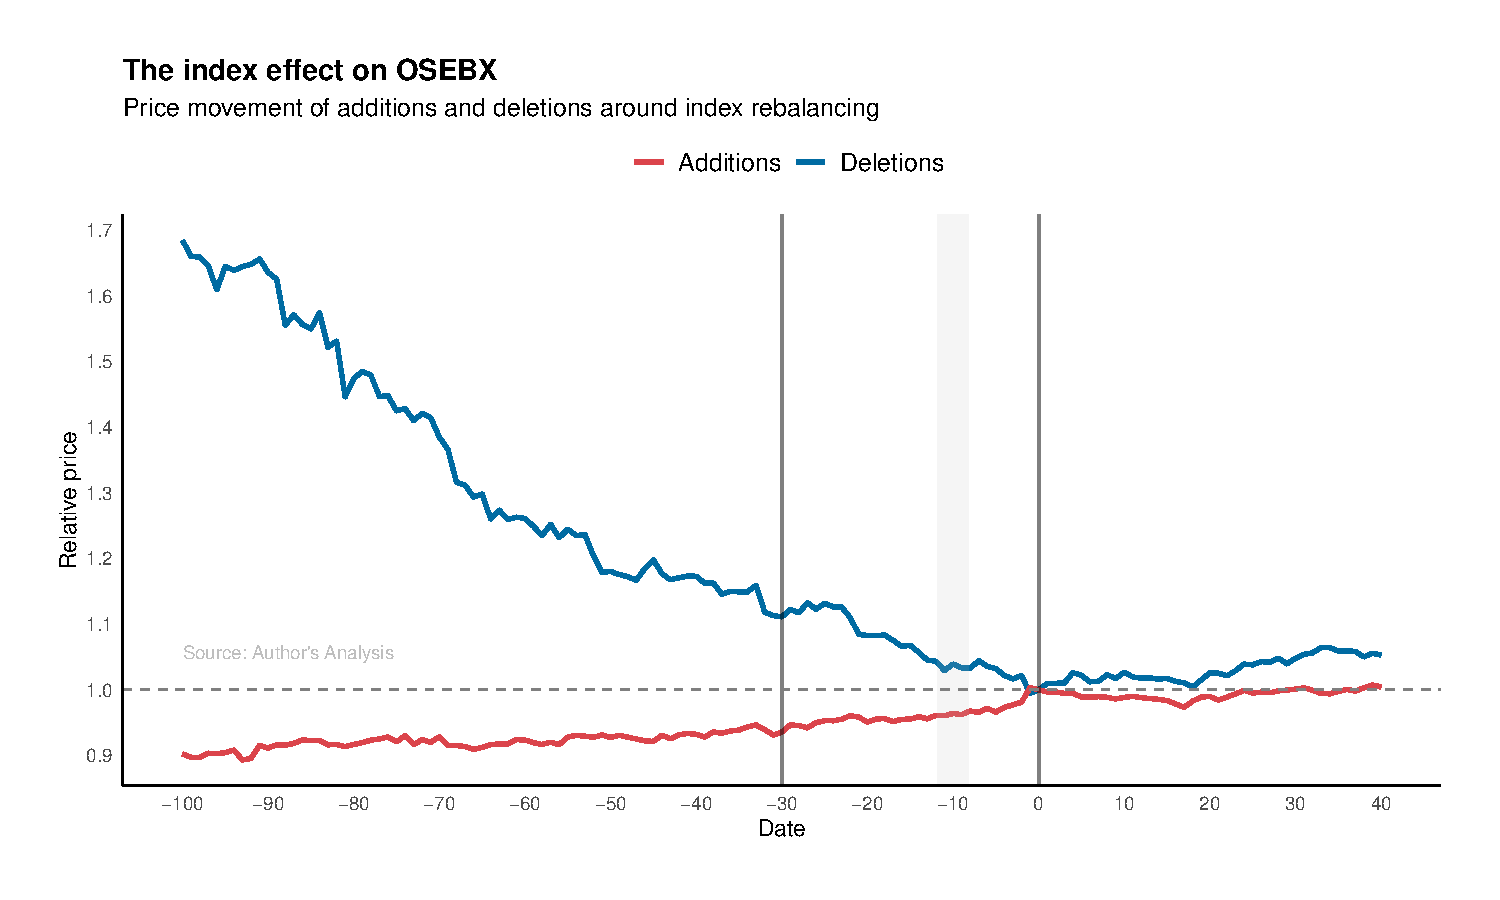
\includegraphics[width=0.95\linewidth]{images/index_plot_updated.pdf}
\caption{\textbf{The index effect on OSEBX, 2002--2023.} Aggregated relative price movements of additions (entering the index) and deletions (leaving the index) in the days surrounding the effective date (day 0). The data cut-off date sits roughly 30 days before ED and the announcement date roughly 14 days before ED. Computed from Bloomberg VWAP data.}
\label{fig:idxeff}
\end{figure}

This paper makes three contributions. First, we frame the index-rebalancing problem as a \emph{conditional} binary classification problem in which the per-firm prior of remaining on (or off) the index is highly asymmetric, and we propose a conditional posterior-probability threshold that exploits this prior. Second, we benchmark a logistic GLM against XGBoost on the four publicly-disclosed Euronext selection variables, demonstrating that 92--95\% classification accuracy is attainable up to 100 trading days before ED. Third, we run a 13-year out-of-sample portfolio simulation under realistic transaction costs and short-borrow assumptions in two settings --- (i) an active long--short overlay and (ii) an enhanced-index sleeve constrained to a 2\% annual tracking error \parencite{ssg-tracking-error-enhanced} --- and obtain Fama--French three-factor alphas significant at the 5\% and 10\% levels respectively. The key empirical takeaway is a sharp trade-off between accuracy and exploitability: the most accurate model is the trivial one (predict no change) and is therefore useless for trading.
